\documentclass[aps,prxquantum,twocolumn,superscriptaddress,floatfix,longbibliography]{revtex4-2}

\usepackage{graphicx}
\usepackage{amsmath,amssymb}
\usepackage{bm}
\usepackage{braket}
\usepackage[colorlinks=true,allcolors=blue]{hyperref}

\graphicspath{{../results/}}

\newcommand{\CR}{\mathcal{C}_R}
\newcommand{\Ztwo}{\mathbb{Z}_2}

\begin{document}

\title{Supplemental Material:\\ Chaotic states outperform quantum many-body
scars as codes under measurement}

\author{Hikaru Wakaura}
\affiliation{QIRI (Quantum Integrated Research Institute Inc.), Tokyo 107-0061, Japan}
\author{Taiki Tanimae}
\affiliation{QIRI (Quantum Integrated Research Institute Inc.), Tokyo 107-0061, Japan}

\date{\today}
\maketitle

\renewcommand{\thesection}{S\arabic{section}}
\renewcommand{\theequation}{S\arabic{equation}}
\renewcommand{\thefigure}{S\arabic{figure}}
\renewcommand{\thetable}{S\arabic{table}}
\setcounter{figure}{0}\setcounter{equation}{0}\setcounter{table}{0}

\section{Constrained basis, PXP spectrum, and scar identification}

The PXP chain is diagonalized in the Rydberg-blockaded basis of bit strings with
no two adjacent excitations (dimension $F(L{+}2)$, Fibonacci; open boundaries).
We benchmark the implementation against the canonical $\Ztwo$-N\'eel revival:
for $L=12$ the return fidelity $|\langle\Ztwo|e^{-iHt}|\Ztwo\rangle|^2$ peaks at
$t\simeq4.70$ with height $0.743$, reproducing the literature. The $L{+}1$
scar-tower eigenstates are selected as the states with anomalously large
$|\langle\Ztwo|E_k\rangle|^2$; the tower forms an approximately equally spaced
ladder at $E\simeq0,\pm1.33,\pm2.66,\pm4.0$. PXP possesses an exponentially large
$E=0$ degeneracy ($8,13,21$ zero modes at $L=10,12,14$); scar and thermal codes
are therefore built from positive-energy rungs ($|E|>0.8$) to avoid this
manifold.

\section{Monitored-trajectory algorithm}

A logical qubit maximally entangled with a reference $R$ is stored as
$\phi\in\mathbb{C}^{d\times2}$, with column $r$ holding $\langle r_R|\Psi\rangle$
(an unnormalized system vector of dimension $d$). Each step applies the dense
propagator $U=e^{-iH\,dt}$ to both columns and then, with probability $p$,
performs a projective measurement: for a diagonal operator with values $\{v\}$ we
Born-sample an eigenvalue from weights $\sum_r\sum_{q:v_q=v}|\phi_{qr}|^2$ and
project. The reference density matrix is $\rho_R=\phi^\dagger\phi$ (a $2\times2$
Hermitian matrix of unit trace), and $S_R=-\mathrm{Tr}\,\rho_R\log_2\rho_R$. We
report $\CR=\langle S_R\rangle$ over $120$--$400$ Born-sampled trajectories with
fixed seeds; error bars are the standard error over trajectories. As a
consistency check, $p=0$ yields $\CR=1$ identically (a unitary on the system
cannot reduce the reference entanglement), and $\CR\to0$ at large $p$.

For a general (non-diagonal) Hermitian measurement operator $O$ (e.g.\ the su(2)
Casimir $J^2$) we precompute its eigenbasis once, rotate $\phi$ into it, project
onto a Born-sampled eigenvalue group, and rotate back.

\section{Thermal-ensemble baseline and the single-pair artifact}

The thermal baseline must be averaged over many energy-matched thermal pairs.
The naive choice---the single non-scar eigenstate nearest each scar-rung
energy---is systematically biased toward atypical, near-scar states with
anomalously low $\CR$. At $L=14$, $p=0.10$, collective monitoring, that single
pair gives $\CR=0.53$, which sits at the $0$th percentile of a $20$-pair
ensemble whose mean is $0.87\pm0.03$ (minimum $0.81$). Averaging over the
ensemble reverses the sign of $\Delta\CR$ and is essential to the conclusion;
all results in the main text use the ensemble baseline.

\section{Static Knill--Laflamme diagnostics}

For a code $\{\ket{0_L},\ket{1_L}\}$ and error set $\{E_a\}$ we quantify
correctability through the logical leak $u_a=\langle0_L|E_a|1_L\rangle$ and
distinguishability $d_a=\langle0_L|E_a|0_L\rangle-\langle1_L|E_a|1_L\rangle$.
Under the local-$Z$ set, energy-matched scar codes have a larger root-mean-square
violation than thermal codes (ratio $1.4$--$2.4$ for $L=10$--$14$), consistent
with ETH-based approximate error correction. Under the collective staggered
operator $M=\sum_i(-1)^iZ_i$ the scar rungs, being connected by the emergent
su(2) generator, carry a large leak $|\langle0_L|M|1_L\rangle|=1.73$ (versus
$\approx0$ for thermal codes), which drives the strong scar penalty under
SGA-aligned monitoring.

The two channels of the main-text criterion are diagnostically distinct. The
diagonal outcome-distribution overlap alone---the Bhattacharyya coefficient
$\mathrm{BC}=\sum_o\sqrt{P_0(o)P_1(o)}$ of the two logical states under the
collective $M$---does \emph{not} predict $\CR$ (Fig.~\ref{fig:supp_bc}): the
scar has a high overlap $\mathrm{BC}=0.96$ yet is poorly protected, because its
$M$-fragility comes from channel (ii), the off-diagonal leak, which $\mathrm{BC}$
cannot see. Both channels are therefore required; no single scalar
(participation, variance, or leak alone) predicts protection across all codes.

\begin{figure}[t]
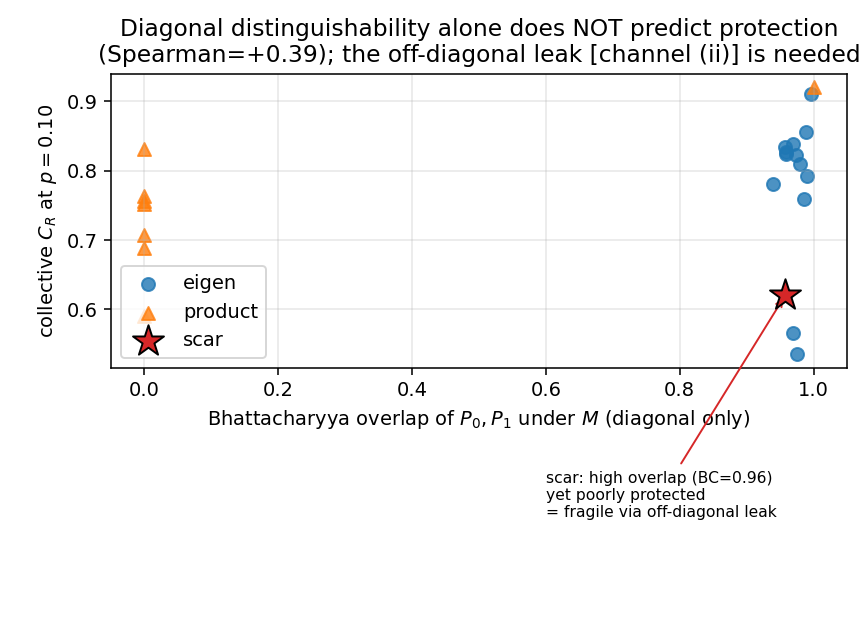
\includegraphics[width=\linewidth]{bhattacharyya.png}
\caption{Collective $\CR$ versus the diagonal Bhattacharyya overlap of the two
logical states under $M$ ($L=14$). The scar (star) has near-unit overlap yet low
$\CR$: its fragility is off-diagonal [channel (ii)], invisible to $\mathrm{BC}$.}
\label{fig:supp_bc}
\end{figure}

\section{Measurement-support phase diagram}

Figure~\ref{fig:supp_pd} maps $\Delta\CR(p,\ell)$ where $\ell$ is the support
size of a block-sum measurement $\sum_{i\in W}Z_i$ over a random contiguous
window $W$ of $\ell$ sites ($\ell{=}1$ local, $\ell{=}L$ global uniform), holding
the per-step event count fixed. Against the ensemble thermal baseline it is
negative throughout: the scar code never wins, and the disadvantage deepens with
both $p$ and $\ell$. (The staggered SGA operator of the main text produces a
larger penalty than the uniform-type block sum because the latter has vanishing
logical leak on the scar rungs.)

\begin{figure}[t]
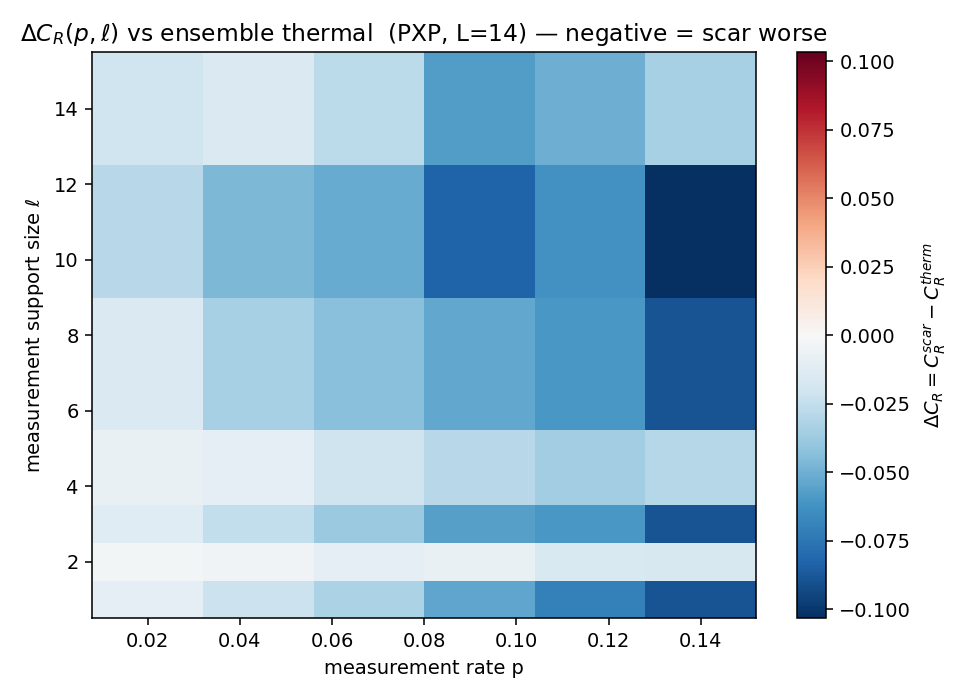
\includegraphics[width=\linewidth]{phase_diagram_L14.png}
\caption{$\Delta\CR(p,\ell)$ against the ensemble thermal baseline (PXP, $L=14$).
Blue is $\Delta\CR<0$ (scar worse) everywhere.}
\label{fig:supp_pd}
\end{figure}

\section{Calibration of the measurement rate}

To connect our discrete per-step rate to the continuous-time rate of
Ref.~[Paviglianiti \& Silva], we reproduce the monitored-N\'eel entanglement
transition (Fig.~\ref{fig:supp_gamma}) and identify the volume-to-area crossing
$p_c\simeq0.05$. With $\gamma=p/dt$ and $dt=0.6$ this gives $\gamma_c\simeq0.083$,
the same order as the reported $\gamma_c\simeq0.013\pm0.002$; the factor
$\sim6$ reflects protocol and estimator differences (stroboscopic per-step
versus continuous-time monitoring; a crossing estimate versus finite-size
scaling) that we have not converted quantitatively.

\begin{figure}[t]
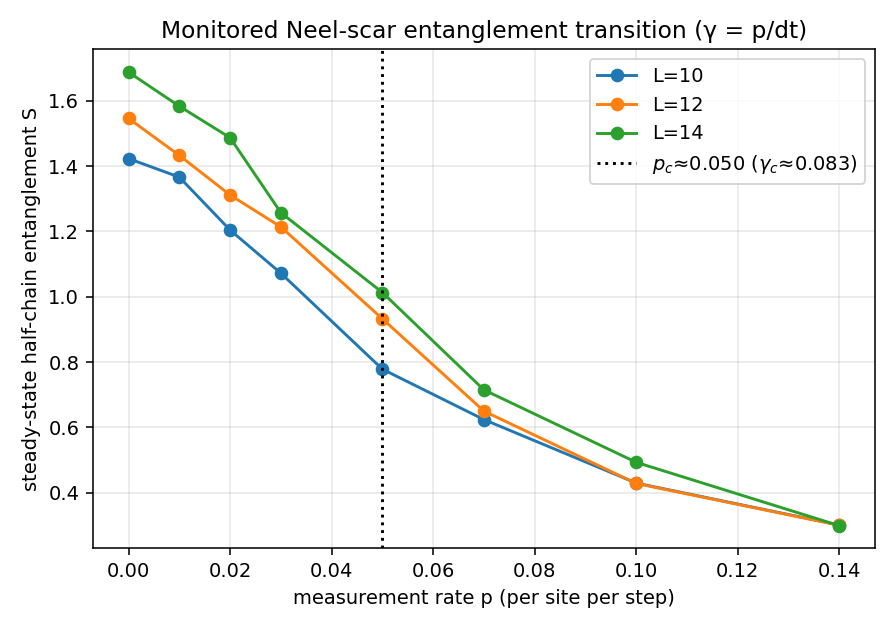
\includegraphics[width=\linewidth]{gamma_mapping.png}
\caption{Steady-state half-chain entanglement of the monitored N\'eel state
versus $p$ for $L=10,12,14$; the crossing sets $p_c$ and hence $\gamma_c=p_c/dt$.}
\label{fig:supp_gamma}
\end{figure}

\section{Spin-1 Schecter--Iadecola model}

The second model is the spin-1 chain
\begin{equation}
H = J\sum_i\!\big(S^x_iS^x_{i+1}+S^y_iS^y_{i+1}\big)
   + h\sum_i S^z_i + D\sum_i (S^z_i)^2,
\end{equation}
with $J{=}1$, $h{=}1$, $D{=}0.1$. Its exact scar tower is
$\ket{S_n}=(Q^+)^n\ket{\Omega}$, $Q^+=\sum_j(-1)^j(S^+_j)^2$,
$\ket{\Omega}=\ket{m{=}{-}1}^{\otimes L}$. The site operators
$\{\ket{m{=}{-}1},\ket{m{=}{+}1}\}$ realize a pseudospin-$\tfrac12$ (with
$\ket{m{=}0}$ outside), and the tower is the fully symmetric Dicke multiplet of
total pseudospin $J=L/2$. With the properly normalized generators
$J^+=Q^+/2$, $J^-=(J^+)^\dagger$, $J^z=\tfrac12\sum_iS^z_i$ one has
$[J^z,J^\pm]=\pm J^\pm$, $[J^+,J^-]=2J^z$, so the Casimir
$J^2=(J^z)^2+\tfrac12(J^+J^-+J^-J^+)$ equals $J(J{+}1)=\tfrac{L}{2}(\tfrac{L}{2}{+}1)$.

We verify numerically that $\ket{S_n}$ are exact eigenstates (residual
$\|H\ket{S_n}-E_n\ket{S_n}\|\sim10^{-16}$), equally spaced by $2$, and that $J^2$
is constant on the tower with variance $\sim10^{-13}$ on every scar---versus
$\mathrm{Var}\,J^2\simeq32$ for PXP scars. Consequently a two-rung scar code has
identical $J^2$ outcome distributions and is an exact decoherence-free subspace
of a $J^2$ measurement, which is why the rescue succeeds here and fails for PXP
($\CR^{\rm scar}=1$, $\Delta\CR=+0.6$ to $+0.9$ at $L=6,8$). Under generic local
$S^z$ monitoring, by contrast, neither code is systematically protected:
$\Delta\CR=+0.10,+0.06,-0.02$ at $p=0.04,0.08,0.12$ (ensemble SEM $\sim0.04$;
$20$-pair ensemble, $L=6$) is scar-favorable at the lowest rate (about
$2\sigma$; up to $+0.17$ at $L=8$) but decays and reverses sign with increasing
$p$, so the scar advantage remains confined to the fine-tuned Casimir probe.

\section{A single-shot resolvability predictor}

The two channels of the main-text criterion combine into one exact,
simulation-free scalar: the reference entropy that survives a \emph{single}
projective $O$-measurement of the freshly encoded pair,
\begin{equation}
s_1(O)=\sum_g q_g\, S\!\big(\rho_R^{(g)}\big),\qquad
\big[\rho_R^{(g)}\big]_{ab} = \frac{\langle b_L|\Pi_g|a_L\rangle}{2q_g},
\end{equation}
with $\Pi_g$ the spectral projectors of $O$ and $q_g=\tfrac12(\langle
0_L|\Pi_g|0_L\rangle+\langle1_L|\Pi_g|1_L\rangle)$ the Born weights. By
construction $s_1=1$ iff a single shot leaves the qubit perfectly
recoverable---the Knill--Laflamme conditions for the projector set
$\{\Pi_g\}$, of which a common-eigenvalue eigenspace (a true DFS) is the
simplest realization---and $s_1=0$ iff one shot fully reads the qubit out;
eigenvalue distinguishability [channel (i)] and non-invariance [channel (ii)]
both enter automatically.

Across $65$ code--measurement pairs spanning both models and five global
operators (Fig.~\ref{fig:supp_pred}), $s_1$ strongly predicts the monitored
$\CR$ \emph{within each resolving measurement}: Spearman $\rho=+0.85$ (PXP,
staggered), $+0.87$ and $+0.81$ (spin-1, Casimir and staggered). Its two
failure modes delimit its scope and are themselves instructive: for a
non-resolving operator (PXP uniform, $s_1\approx1$ for all codes) there is no
signal left to predict, and for an operator that does not commute with the
Hamiltonian (the PXP Casimir, $[J^2,H]\neq0$) the dynamics between shots dress
the resolvability and shift $\CR$ systematically below the single-shot
estimate. We therefore present $s_1$ as an operational design quantity---an
exact, Monte-Carlo-free screen for candidate code/measurement pairs---rather
than a universal collapse variable.

\begin{figure}[t]
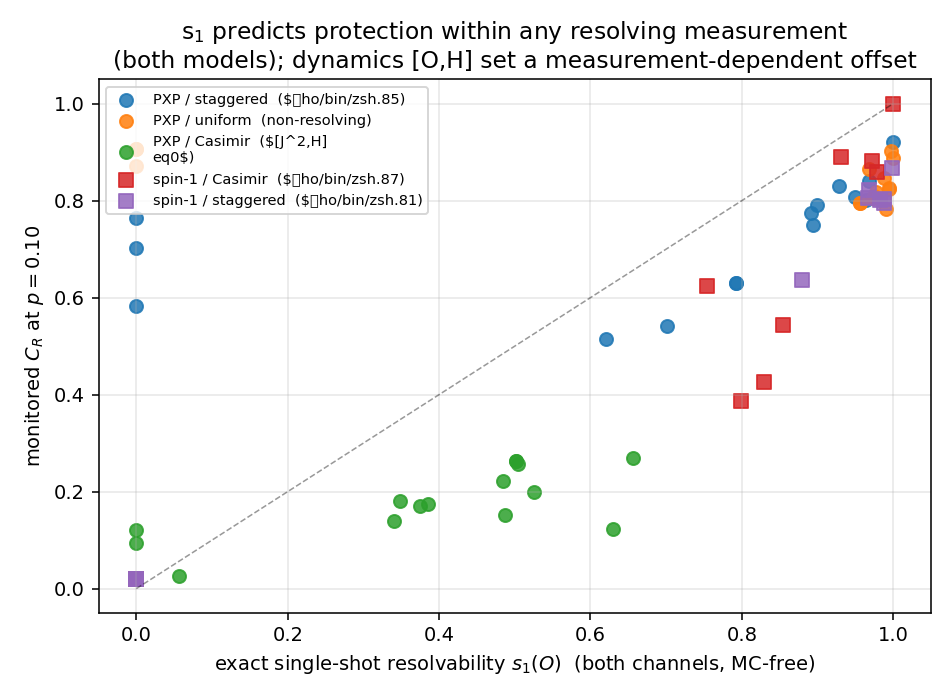
\includegraphics[width=\linewidth]{predictor.png}
\caption{Monitored $\CR$ ($p=0.10$) versus the exact single-shot resolvability
$s_1(O)$ for $65$ code--measurement pairs across both models. Within each
resolving measurement the relation is tight; the non-resolving (uniform) and
non-commuting (PXP Casimir) families bound the predictor's scope.}
\label{fig:supp_pred}
\end{figure}

\section{Extensive code under collective and Casimir monitoring}

The maximal $k=\lfloor\log_2(L{+}1)\rfloor$-qubit scar code of the main text is
compared to a same-dimension thermal code under all three PXP measurement models
in Table~\ref{tab:ext} ($L=14$, $k=3$, protected density $S_R/k$, $8$-draw
thermal ensemble). The pattern matches the single-qubit analysis: the scar loses
under local and (strongly) collective monitoring and is only comparable under
the fine-tuned Casimir.

\begin{table}[h]
\caption{Extensive-code density gap $\Delta(S_R/k)=$ scar $-$ thermal ($L=14$,
$k=3$).}
\label{tab:ext}
\begin{ruledtabular}
\begin{tabular}{lccc}
measurement & $p{=}0.04$ & $p{=}0.08$ & $p{=}0.12$ \\
\colrule
local $S^z$    & $-0.14$ & $-0.06$ & --- \\
collective $M$ & $-0.32$ & $-0.40$ & $-0.43$ \\
Casimir $J^2$  & $+0.02$ & $+0.03$ & $+0.03$ \\
\end{tabular}
\end{ruledtabular}
\end{table}

\end{document}
